% LOOM - camera-ready in the Hinweis Research (HR) template: single column, A4, Times, 9 pt text,
% margins top/bottom 3.25 cm, left 3 cm, right 2.5 cm, no paragraph indent, no page numbers, no screenshots.
\documentclass[9pt,a4paper]{extarticle}
\usepackage[a4paper,top=3.25cm,bottom=3.25cm,left=3cm,right=2.5cm,headheight=0pt,headsep=0pt,footskip=0.36cm]{geometry}
\usepackage[T1]{fontenc}
\usepackage{newtxtext,newtxmath}
\usepackage{amsmath}
\usepackage{graphicx}
\usepackage{array}
\usepackage{xcolor}
\usepackage{algorithm}
\usepackage{algpseudocode}
\usepackage{tikz}
\usetikzlibrary{arrows.meta,positioning,fit,calc,backgrounds,patterns,shapes.geometric}
\usepackage{titlesec}
\usepackage[font=footnotesize,labelsep=period]{caption}
\usepackage{enumitem}
\usepackage{microtype}
\usepackage[hidelinks]{hyperref}
\usepackage{url}

\definecolor{lsky}{HTML}{2F7FC1}
\definecolor{lmint}{HTML}{1E9E7E}
\definecolor{lpeach}{HTML}{E07A45}
\definecolor{llilac}{HTML}{7B5CD6}
\definecolor{lcoral}{HTML}{D6455F}
\definecolor{lgrey}{HTML}{5B6B78}

% paragraphs: single spaced, no indent, no space between paragraphs
\setlength{\parindent}{0pt}
\setlength{\parskip}{0pt}
\pagestyle{empty}
% headings: "I. INTRODUCTION" (10 pt, small caps), 12 pt before / 6 pt after;
% subheadings "A. Title" (9 pt italic), 6 pt before / 3 pt after
\renewcommand\thesection{\Roman{section}}
\renewcommand\thesubsection{\Alph{subsection}}
\titleformat{\section}{\fontsize{10}{12}\selectfont}{\thesection.}{0.5em}{\scshape}
\titlespacing*{\section}{0pt}{12pt}{6pt}
\titleformat{\subsection}{\fontsize{9}{11}\selectfont\itshape}{\thesubsection.}{0.5em}{}
\titlespacing*{\subsection}{0pt}{6pt}{3pt}
\titleformat{name=\section,numberless}{\fontsize{10}{12}\selectfont}{}{0pt}{\scshape}
% captions: "Figure 1." below figures, "TABLE I." (small caps) above tables, centred, 8 pt
\captionsetup[figure]{name=Figure,justification=centering}
\captionsetup[table]{name=TABLE,justification=centering,font={footnotesize,sc},skip=4pt}
\renewcommand\thetable{\Roman{table}}
\setlength{\textfloatsep}{10pt plus 2pt minus 2pt}
\setlength{\abovecaptionskip}{4pt}
\newcolumntype{L}[1]{>{\raggedright\arraybackslash}p{#1}}
\newcommand{\fig}[1]{Fig.~\ref{#1}}
\newcommand{\tab}[1]{Table~\ref{#1}}
\renewcommand{\algorithmicrequire}{\textbf{Input:}}
\renewcommand{\algorithmicensure}{\textbf{Output:}}

\begin{document}

\begin{center}
{\fontsize{20}{24}\selectfont LOOM: A Verified Multi-Agent System for Object-Level\\ Personalization of Instructional Video\par}
\vspace{10pt}
{\fontsize{10}{12}\selectfont Kamal Karteek U$^1$, Manya Ravishankar$^2$, Jeevika R$^3$ and Dr.\ Sangeetha J$^4$\par}
\vspace{2pt}
{\fontsize{9}{11}\selectfont $^{1-4}$Department of Computer Science and Engineering, Ramaiah Institute of Technology, Bengaluru, India\\
Email: 1ms23cs229@msrit.edu, manya7135@gmail.com, 1ms23cs230@msrit.edu, sangeethakirank@msrit.edu\par}
\end{center}
\vspace{6pt}

\begin{list}{}{\leftmargin=1.1cm\rightmargin=1.1cm}\item\relax
\textbf{\textit{Abstract}---One lesson video serves very different viewers: an expert who wants the new idea without
the setup, a beginner who needs the missing prerequisite, and a parent who wants the broken glass in a chemistry
demonstration hidden from a child. Today each of them gets the same file. We present LOOM, a system that turns one
source video into a different cut for every viewer and delivers a cut only after an independent Critic has verified it.
A one-time perception pass builds a shared lesson graph of speech, on-screen text, tracked objects with pixel masks,
board elements, concepts and verified quiz questions. Six cooperating agents then plan a cut per viewer inside a
bounded repair loop that falls back to a conservative cut when verification fails. Hazards are hidden as objects, not
by blocking the lesson: an open-vocabulary detector proposes them, and a hazard is kept when an image--text verifier
or a vision-language check confirms it. Everything runs on one 8\,GB laptop GPU. On a lesson with known hazard timing,
verification cuts false blocking from 30.1\,s to 0.5\,s at a recall of 0.80, below our 0.90 target. The Critic detects
all 76 planted faults and approves all 9 clean cuts, a verified cut is built in 0.27\,s, and a 22-lesson run over 12
teaching styles shows the pipeline running end to end beyond the corpus. We report every parameter, the failure cases
and the ethical limits of the design.}

\vspace{6pt}
\textbf{\textit{Index Terms}---multi-agent systems, personalized video learning, object-level redaction,
open-vocabulary grounding, verification loops, fail-closed safety, local language models.}
\end{list}

\section{Introduction}
A lesson video is recorded once and watched by many people with different needs. An expert wants the ten-minute version
of a thirty-minute lecture. A beginner needs the prerequisite the lecturer skipped. A parent who lets a child watch a
chemistry demonstration wants the shattering bottle hidden, not the whole lesson. The options a viewer has today are
coarse: watch everything, scrub around, or accept one age rating for the entire clip. Adaptive-learning research
personalises the learning path or the presentation of content [1], [2], hypervideo adds interactive links inside a
video [3], and content classifiers do look inside videos, but they label a clip or a frame as a whole [4], [5].

LOOM (Live, Object-grounded, Orchestrated Media) takes a different position: \emph{one source video, a different
verified cut per viewer}. A cut selects, shortens or expands parts of the lesson, attaches explainers and a quiz, and
hides specific objects in specific seconds. The cut is checked before it is played; if it cannot be verified within a
small budget, the system fails closed and plays a conservative cut instead of its best guess. All models run locally on
a single 8\,GB laptop GPU, so lesson footage and learner data stay on the machine.

The contributions are: (1) a one-time perception pipeline that builds a shared lesson graph of transcript, on-screen
text, tracked objects with pixel masks, board and animation elements, concepts and verified quiz questions, including a
board memory that sees through the teacher and separates burned-in captions from the board; (2) a mesh of six agents in
a Perceive--Plan--Act--Verify loop with a Critic that is separate from the planners, a bounded budget and a fail-closed
fallback, with three further services reached through the Agent2Agent (A2A) protocol [6]; (3) object-level,
viewer-specific redaction from two complementary safety paths, verified hazard classes and a per-object safety review;
(4) generated explainers planned in a constrained scene language, with exact geometry for compass-and-straightedge
constructions and a line-by-line fact-check whose verdicts are shown to the learner; and (5) an evaluation with a
per-rule hazard ablation, time-padding sweeps, fault injection, repeated-run latency, a 22-lesson breadth run and the
complete parameter set.

We ask five research questions. \emph{RQ1}: can per-viewer verified cuts be produced fully locally within a bounded
number of repair passes? \emph{RQ2}: does staged verification make object-level redaction practical? \emph{RQ3}: does a
constrained scene language produce correct explainers where free-form animation code fails? \emph{RQ4}: does staged
fact-checking keep unsupported narration out of explainers? \emph{RQ5}: can retrieval and orchestration stay
inspectable to the viewer?

\section{Related Work}
\subsection{Adaptive and Interactive Video}
Sanal Kumar and Thandeeswaran propose an adaptive personalisation model for video-based e-learning [1]; Hardaker and
Glenn review AI for personalised learning [2]; Cattaneo \emph{et al.} give a design model for hypervideo [3]. These
adapt the path through content. LOOM edits the video itself: it selects, condenses or expands segments, hides objects
and checks the result before delivery.

\subsection{Language-Model Agents for Learning}
GenMentor maps a learner's goal to skills and a learning path with several agents [7], EduPlanner uses evaluator,
optimizer and analyst agents to improve lesson plans [8], and PAL turns lecture videos into interactive sessions [9].
Self-Refine shows that a model can improve its own output from feedback [10], and language-model judges are widely
used to grade generated text [11]. LOOM's loop differs in three ways: the checker is separate from the producers
(deterministic rules plus a judge model from a different family and a dedicated safety model), the budget is bounded,
and exhausting it yields a safe fallback rather than the last draft.

\subsection{Inappropriate-Content Detection}
Chuttur and Nazurally detect inappropriate cartoon video with a multi-modal approach [4], and Yousaf and Nawaz classify
inappropriate YouTube videos [5]. Their output is a label for the clip. A parent needs more: which object, in which
seconds, at which pixels, with the rest of the lesson intact. \tab{tab:compare} summarises the difference.

\begin{table}[t]
\caption{Comparison with the closest systems}
\label{tab:compare}
\centering
\begin{tabular}{|l|l|c|c|c|}
\hline
System & Output & Agents & Hides objects & Verifies own output\\
\hline
PAL [9] & Interactive sessions & -- & -- & --\\
GenMentor [7] & Learning path, content & yes & -- & --\\
EduPlanner [8] & Lesson plans & yes & -- & yes\\
Hypervideo [3] & Design model & -- & -- & --\\
Moderation [4], [5] & Clip label & -- & -- & --\\
\textbf{LOOM} & Per-viewer cut & yes & yes & yes\\
\hline
\end{tabular}
\end{table}

\section{Problem Formulation}
A lesson is a video $V$ of duration $D$. Perception maps it once to a graph $G=(S,X,O,K,Q)$: transcript sentences $S$,
on-screen text spans $X$, tracked objects $O$ (each with instances, a box and a pixel mask per sample, and a safety
review), concepts $K$ with prerequisite edges and evidence links to $S$ and $X$, and a verified quiz bank $Q$. A viewer
$v$ has a mastery $m_v(k)\in[0,1]$ per concept, a pace and a safety profile. A \emph{cut} $C$ is an ordered set of
non-overlapping intervals of $V$, each with an action (keep, condense, expand), plus explainer requests and quiz items
from $Q$; a \emph{mask schedule} $M$ lists, per object, the time span and the padded mask to hide.

A pair $(C,M)$ is \emph{verified} for $v$ when a Critic function $I(C,M,G,v)$ returns no issue. Issues cover safety (an
object that must be hidden for $v$ is visible inside $C$ without a mask, checked every 0.1\,s), coherence (an empty or
overlapping cut, a condensed thread that ends mid-sentence, a dropped prerequisite the viewer has not mastered, a
missing explainer), factuality (a quiz item outside $Q$) and completeness (no quiz although $Q$ covers the cut). The
system must return a verified pair, or a fallback whose safety does not depend on any model's judgement.

Hazard redaction is scored in time against a ground-truth hazard window $H$. With $P$ the union of the masked seconds of
hazard objects, both discretised to 0.1\,s ticks,
\begin{equation}
\mathrm{prec}=\frac{|P\cap H|}{|P|}, \qquad \mathrm{rec}=\frac{|P\cap H|}{|H|},
\end{equation}
while the \emph{false-block} time $|P\setminus H|$ is the safe footage hidden and the \emph{missed} time $|H\setminus P|$
is the hazard left visible.

\section{Proposed System}
\subsection{Overview}
\fig{fig:arch} shows the three layers. \emph{Perception} runs once per lesson and may take minutes. The \emph{agent
mesh} builds a cut for a viewer in well under a second, because its agents are deterministic code over the stored
graph. \emph{Services} (retrieval, explainers, topic quizzes) call language models on demand. All models are reached
through Ollama on a loopback address or loaded from cached weights; only a user-initiated YouTube download touches the
network.

\begin{figure}[t]
\centering
\resizebox{\textwidth}{!}{% LOOM architecture: layers as rows, layer names in a left column, arrows away from the labels.
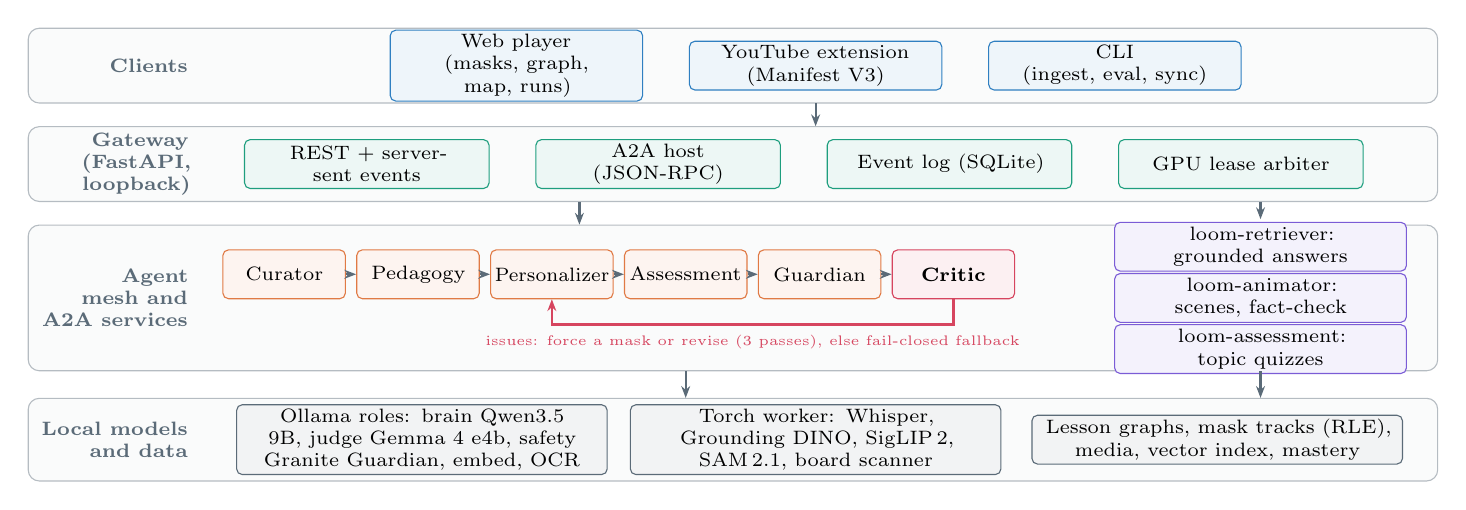
\begin{tikzpicture}[font=\scriptsize,
  box/.style={draw=#1, fill=#1!8, rounded corners=2pt, align=center, minimum height=6.2mm, inner sep=1.5pt},
  arr/.style={-{Stealth[length=1.5mm]}, lgrey, thick},
  layer/.style={draw=lgrey!45, fill=lgrey!3, rounded corners=4pt},
  lname/.style={font=\scriptsize\bfseries, text=lgrey, align=right, text width=1.9cm, anchor=east}]
% layer frames (drawn first)
\foreach \y/\h/\name in {0/0.95/{Clients}, -1.25/0.95/{Gateway\\(FastAPI, loopback)}, -2.95/1.85/{Agent mesh and\\A2A services}, -4.75/1.05/{Local models\\and data}} {
  \draw[layer] (0,\y-\h/2) rectangle (17.9,\y+\h/2);
  \node[lname] at (2.15,\y) {\name};
}
% clients
\node[box=lsky, text width=3.1cm] (web) at (6.2,0) {Web player\\(masks, graph, map, runs)};
\node[box=lsky, text width=3.1cm] (ext) at (10.0,0) {YouTube extension\\(Manifest V3)};
\node[box=lsky, text width=3.1cm] (cli) at (13.8,0) {CLI\\(ingest, eval, sync)};
% gateway
\node[box=lmint, text width=3.0cm] (rest) at (4.3,-1.25) {REST + server-sent events};
\node[box=lmint, text width=3.0cm] (a2a) at (8.0,-1.25) {A2A host\\(JSON-RPC)};
\node[box=lmint, text width=3.0cm] (log) at (11.7,-1.25) {Event log (SQLite)};
\node[box=lmint, text width=3.0cm] (gpu) at (15.4,-1.25) {GPU lease arbiter};
% mesh
\foreach \n/\x/\c in {cur/3.25/Curator, ped/4.95/Pedagogy, per/6.65/Personalizer, ass/8.35/Assessment, gua/10.05/Guardian} {
  \node[box=lpeach, text width=1.45cm] (\n) at (\x,-2.65) {\c};
}
\node[box=lcoral, text width=1.45cm] (cri) at (11.75,-2.65) {\textbf{Critic}};
\draw[arr] (cur) -- (ped); \draw[arr] (ped) -- (per); \draw[arr] (per) -- (ass); \draw[arr] (ass) -- (gua); \draw[arr] (gua) -- (cri);
\draw[arr, lcoral] (cri.south) -- ++(0,-0.32) -| node[pos=0.25, below, text=lcoral, font=\tiny] {issues: force a mask or revise (3 passes), else fail-closed fallback} (per.south);
% A2A services
\node[box=llilac, text width=3.6cm] (ret) at (15.65,-2.3) {loom-retriever: grounded answers};
\node[box=llilac, text width=3.6cm] (ani) at (15.65,-2.95) {loom-animator: scenes, fact-check};
\node[box=llilac, text width=3.6cm] (qz) at (15.65,-3.6) {loom-assessment: topic quizzes};
% models and data
\node[box=lgrey, text width=4.6cm] (oll) at (5.0,-4.75) {Ollama roles: brain Qwen3.5 9B, judge Gemma 4 e4b, safety Granite Guardian, embed, OCR};
\node[box=lgrey, text width=4.6cm] (torch) at (10.0,-4.75) {Torch worker: Whisper, Grounding DINO, SigLIP\,2, SAM\,2.1, board scanner};
\node[box=lgrey, text width=4.6cm] (db) at (15.1,-4.75) {Lesson graphs, mask tracks (RLE), media, vector index, mastery};
% between layers
\draw[arr] (10.0,-0.48) -- (10.0,-0.77);
\draw[arr] (7.0,-1.73) -- (7.0,-2.02);
\draw[arr] (15.65,-1.73) -- (15.65,-1.95);
\draw[arr] (8.35,-3.88) -- (8.35,-4.22);
\draw[arr] (15.65,-3.88) -- (15.65,-4.22);
\end{tikzpicture}
}
\caption{LOOM architecture. Perception runs once per lesson and writes the graph; the deterministic mesh builds and
verifies a cut per viewer; three A2A services answer questions, plan explainers and write topic quizzes on demand}
\label{fig:arch}
\end{figure}

\subsection{Perception Pipeline}
\fig{fig:pipe} lists the stages. After probing and shot detection (PySceneDetect [12]), speech is transcribed with
Whisper large-v3-turbo [13] in 60\,s chunks. On-screen text is read by RapidOCR [14] and re-read by the GLM-OCR model
[25] when its confidence is below 0.85. A vocabulary stage asks the language model which objects matter; twelve hazard
classes (broken glass, knife, blade, scissors, needle, open flame, fire, blood, gun, cigarette, pills, syringe) are
always added. Grounding DINO [15] proposes boxes at 2\,fps, and at 4\,fps inside windows around hazard proposals; an IoU
tracker links them into tracks per shot. A fusion stage, run by the brain model, groups sentences and text into
concepts with prerequisites and evidence links, and the embedding model [16] indexes all of it for retrieval. The
safety stage reviews every tracked object, and a quiz stage writes questions that the judge model must verify before
they enter the bank. Finally SAM\,2.1 [17] turns kept tracks into pixel masks, processed in 20\,s windows at 5\,fps and
480\,px, which lowers peak GPU memory from 8.88\,GB to 2.91\,GB. With 8\,GB of memory one heavy model is resident at a
time, every GPU job goes through a priority arbiter, and torch stages never run while a language model is loaded.

\begin{figure}[t]
\centering
\resizebox{0.97\textwidth}{!}{% Perception pipeline (left to right, two rows) and the hazard-verification branch; black-and-white friendly.
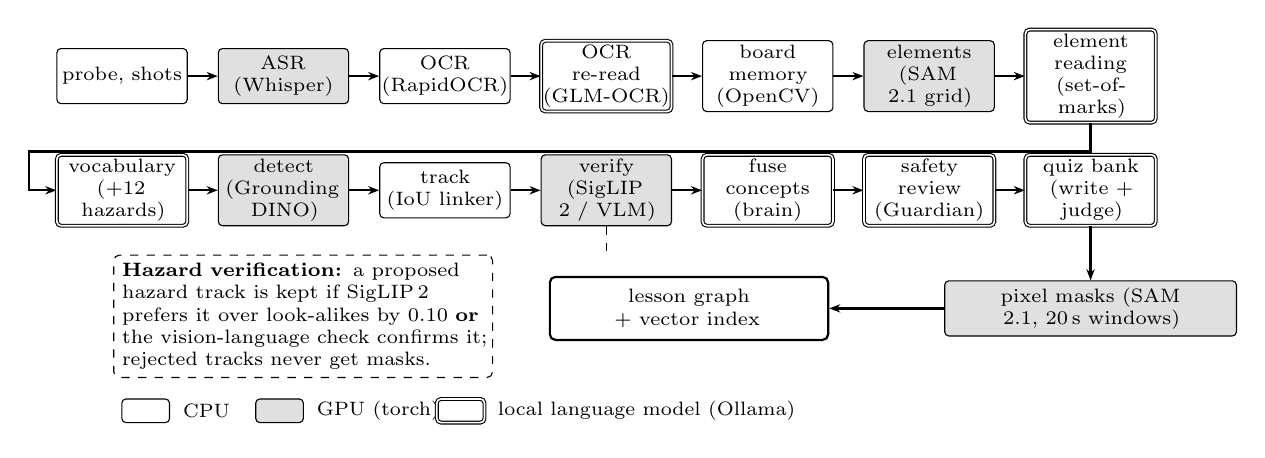
\begin{tikzpicture}[font=\scriptsize,
  st/.style={draw, rounded corners=1.5pt, align=center, minimum height=7mm, text width=1.55cm, inner sep=1.5pt},
  gpu/.style={st, fill=black!12},
  llm/.style={st, fill=white, double},
  arr/.style={-{Stealth[length=1.4mm]}, thick}]
\node[st]  (probe) at (0,0)    {probe, shots};
\node[gpu] (asr)   at (2.05,0) {ASR\\(Whisper)};
\node[st]  (ocr)   at (4.1,0)  {OCR\\(RapidOCR)};
\node[llm] (rer)   at (6.15,0) {OCR re-read\\(GLM-OCR)};
\node[st]  (board) at (8.2,0)  {board memory\\(OpenCV)};
\node[gpu] (elem)  at (10.25,0) {elements\\(SAM 2.1 grid)};
\node[llm] (bread) at (12.3,0) {element reading\\(set-of-marks)};
\node[llm] (voc)   at (0,-1.45)   {vocabulary\\(+12 hazards)};
\node[gpu] (det)   at (2.05,-1.45) {detect\\(Grounding DINO)};
\node[st]  (trk)   at (4.1,-1.45)  {track\\(IoU linker)};
\node[gpu] (ver)   at (6.15,-1.45) {verify\\(SigLIP 2 / VLM)};
\node[llm] (fuse)  at (8.2,-1.45)  {fuse concepts\\(brain)};
\node[llm] (safe)  at (10.25,-1.45) {safety review\\(Guardian)};
\node[llm] (quiz)  at (12.3,-1.45) {quiz bank\\(write + judge)};
\node[gpu, text width=3.6cm] (sam) at (12.3,-2.95) {pixel masks (SAM 2.1, 20\,s windows)};
\node[draw, thick, rounded corners=2pt, text width=3.3cm, align=center, minimum height=8mm] (graph) at (7.2,-2.95) {lesson graph + vector index};
\foreach \a/\b in {probe/asr, asr/ocr, ocr/rer, rer/board, board/elem, elem/bread, voc/det, det/trk, trk/ver, ver/fuse, fuse/safe, safe/quiz} \draw[arr] (\a) -- (\b);
\draw[arr] (bread.south) -- ++(0,-0.36) -| ($(voc.west)+(-0.35,0)$) -- (voc.west);
\draw[arr] (quiz) -- (sam);
\draw[arr] (sam) -- (graph);
% verification detail
\node[draw, dashed, rounded corners=2pt, align=left, text width=4.6cm, inner sep=3pt] (vd) at (2.3,-3.05)
  {\textbf{Hazard verification:} a proposed hazard track is kept if SigLIP\,2 prefers it over look-alikes by 0.10 \textbf{or} the vision-language check confirms it; rejected tracks never get masks.};
\draw[dashed] (ver.south) -- (vd.north -| ver.south);
% legend
\node[st, text width=0.5cm, minimum height=3mm] at (0.3,-4.25) {}; \node[anchor=west] at (0.65,-4.25) {CPU};
\node[gpu, text width=0.5cm, minimum height=3mm] at (2.0,-4.25) {}; \node[anchor=west] at (2.35,-4.25) {GPU (torch)};
\node[llm, text width=0.5cm, minimum height=3mm] at (4.3,-4.25) {}; \node[anchor=west] at (4.65,-4.25) {local language model (Ollama)};
\end{tikzpicture}
}
\caption{Perception stages, run once per lesson, and the hazard-verification rule}
\label{fig:pipe}
\end{figure}

\subsection{Hazard Verification and Masking}
The detector is deliberately generous: on the demo lesson it proposes 30 hazard tracks, most of them wrong (a beaker as
``broken glass''). A track is kept when SigLIP\,2 [18] prefers the hazard phrase over a curated list of look-alikes (a
glass beaker or a bottle for broken glass) by a margin of 0.10, \emph{or} when a vision-language crop check confirms it.
The OR rule is deliberate: each verifier can only add a hazard, never veto the other, because a missed hazard costs more
than a masked beaker.

Independently, Granite Guardian [19] reviews every tracked object, whatever its class, against a nine-category taxonomy
(sharp object, injury risk, fire or explosion, weapon, blood or gore, nudity, drugs or alcohol, hazardous chemical,
disturbing). A viewer's safety profile decides what is hidden: the Parent\,+\,child profile masks objects reviewed as
unsafe for a child with severity of at least 0.5, a strict profile lowers the threshold to 0.2, and any object whose
review did not complete is masked. This second path matters: it is the one that catches a broken glass pipette lying on
a laboratory floor (Section VI-\ref{sec:second}). Masks are padded by 0.5\,s in time and by 0.04 of the box in space, three
times wider for child-unsafe objects.

\subsection{Board and Animation Elements}
Many lessons are drawn on a board or animated, so there is no physical object to detect. An OpenCV \emph{board memory}
updates a pixel only where the board is visible in two agreeing samples, so a teacher standing in front never erases
the writing; it tolerates a shaking phone camera, picks the board as the surface that carries the ink rather than the
largest one, and splits long strokes so a border does not swallow a diagram. Because it remembers the last unobstructed
colour of every board pixel, the player can render the teacher see-through. Burned-in captions are told apart from the
board because they keep their colour while what lies beneath them changes. On drawn frames, SAM\,2.1's point-grid mask
generator (0.6--0.7\,s per frame, 2.4\,GB) finds elements and their parts, and one set-of-marks call [20] names all the
numbered parts of an element at once.

\subsection{Agent Mesh and Personalisation Rules}
Six agents run in-process. The \emph{Curator} cuts the lesson into threads at sentence boundaries. The \emph{Pedagogy}
agent assigns each thread an action from the viewer's mastery $m$ of its concepts: skip if $m\geq0.80$, condense if
$m\geq0.60$, keep if $m\geq0.35$, otherwise expand; the pace adds $-0.10$, $0$ or $+0.10$, and a prerequisite whose
mastery is below 0.35 is never dropped. The \emph{Personalizer} builds the timeline: a condensed thread keeps the larger
of 6\,s and half its length, ends on a sentence boundary, and holds an on-screen formula for 3\,s. The \emph{Assessment}
agent picks up to three verified questions and later updates mastery ($+0.35$ for a correct answer, $\times0.75$ for a
wrong one, $+0.05$ per explainer, $+0.03$ per exposure). The \emph{Guardian} builds the mask schedule for the profile,
and the \emph{Critic} computes $I(C,M,G,v)$ and four scores (safety, coherence, factuality, completeness) that are shown
to the viewer.

\subsection{Verification Loop and Fail-Closed Behaviour}
Algorithm~\ref{alg:loop} gives the loop. A cut is approved only when the Critic finds no issue at all. An unmasked
hazard is repaired locally by forcing a mask; structural issues (an overlap, a cut mid-sentence, a dropped
prerequisite, a missing explainer) go back to the mesh. After three passes the viewer receives the \emph{fallback cut}:
the whole lesson, no generated content, and every object masked for profiles with redaction on. The same principle
covers model failures: an object whose safety review cannot be completed is masked, an explainer that cannot be
verified is not shown, and a degraded result is never cached.

\begin{algorithm}[t]
\caption{Verify-before-deliver loop}
\label{alg:loop}
\begin{algorithmic}[1]
\Require lesson graph $G$, viewer $v$, budget $B=3$
\Ensure a verified pair $(C,M)$, or the fallback cut
\State $T\gets$ \textsc{Pedagogy}(\textsc{Curator}$(G)$, $v$);\quad $C\gets$ \textsc{Personalize}$(T,v)$
\State $C.quiz\gets$ \textsc{Assessment}$(C,G,v)$;\quad $F\gets\emptyset$ \Comment{masks forced by the Critic}
\For{$p=1$ \textbf{to} $B$}
  \State $M\gets$ \textsc{Guardian}$(G,v,C)\cup F$
  \State $I\gets$ \textsc{Critic}$(C,M,G,v)$
  \If{$I=\emptyset$} \Return $(C,M)$ \Comment{approved}
  \EndIf
  \State $F\gets F\cup\{o : \text{object } o \text{ is an unmasked hazard in } I\}$
  \State $C\gets$ \textsc{Revise}$(C, \{i\in I: i \text{ is routed to the mesh}\})$
\EndFor
\State \Return \textsc{Fallback}$(G,v)$ \Comment{whole lesson, nothing generated, every object masked}
\end{algorithmic}
\end{algorithm}

\subsection{Explainers and Fact-Checking}
When a viewer asks a question, the \emph{loom-animator} service retrieves evidence from the lesson and asks the brain
model for a \emph{scene plan} in a small domain-specific language instead of free-form animation code: beats with one
narrated sentence each, labelled elements and a few actions (appear, move, merge, highlight, connect). A layout solver
places the elements and a three.js player renders the scene with Kokoro-82M narration [21]; Manim [22] only exports a
background MP4. Geometry questions use a second plan type: the model names the construction (points, rays, an arc
centred on a point, the crossing of two arcs) and a solver computes every coordinate exactly, widening compass arcs that
would not meet and opening a degenerate given angle. Steps that do not resolve go back to the planner like a
fact-checker's rejections. \fig{fig:construct} draws the construction that the solver resolved for an angle-bisector
request: all 12 steps resolve, and the two half-angles agree within 0.01$^\circ$.

\begin{figure}[t]
\centering
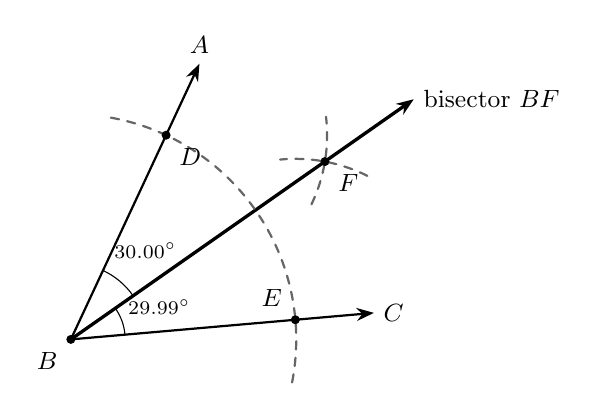
\begin{tikzpicture}[scale=0.92, line cap=round, font=\small]
\tikzset{ray/.style={thick, -{Stealth[length=2.2mm]}}, arc/.style={thick, dashed, black!60}, pt/.style={circle, fill=black, inner sep=1.15pt}}
\draw[ray] (-2.367,-1.106) -- (-0.592,2.700);
\draw[ray] (-2.367,-1.106) -- (1.817,-0.740);
\draw[ray, very thick] (-2.367,-1.106) -- (2.367,2.209);
\draw[arc] (0.687,-1.700) arc[start angle=-11.00, end angle=81.00, radius=3.111];
\draw[arc] (0.955,0.759) arc[start angle=334.57, end angle=366.57, radius=2.222];
\draw[arc] (1.726,1.152) arc[start angle=63.43, end angle=95.43, radius=2.222];
\draw[thin] (-1.620,-1.041) arc[start angle=5.00, end angle=34.99, radius=0.75];
\node[font=\scriptsize] at (-1.145,-0.661) {$29.99^\circ$};
\draw[thin] (-1.507,-0.504) arc[start angle=34.99, end angle=65.00, radius=1.05];
\node[font=\scriptsize] at (-1.338,0.120) {$30.00^\circ$};
\node[pt, label={[font=\small]below left:$B$}] at (-2.367,-1.106) {};
\node[pt, label={[font=\small]below right:$D$}] at (-1.052,1.713) {};
\node[pt, label={[font=\small]above left:$E$}] at (0.732,-0.835) {};
\node[pt, label={[font=\small]below right:$F$}] at (1.140,1.349) {};
\node[font=\small, above] at (-0.592,2.700) {$A$};
\node[font=\small, right] at (1.817,-0.740) {$C$};
\node[font=\small, right] at (2.367,2.209) {bisector $BF$};
\end{tikzpicture}
\caption{The angle-bisector construction as resolved by the solver for ``explain the angle bisector construction step
by step''. Dashed: compass arcs from $B$ (crossing the rays at $D$ and $E$) and equal arcs from $D$ and $E$ (crossing at
$F$). The half-angles are measured from the stored drawing coordinates}
\label{fig:construct}
\end{figure}

Each narrated line is checked against the retrieved evidence by the judge model, Gemma\,4\,e4b [23], followed by two
deterministic rules: a rejection whose only ground is that the evidence does not mention a claim is overruled (the
judge's own instructions forbid it, yet the judge does it for standard procedures), and a line that narrates the video
instead of teaching the topic is rejected. A plan with too many unsupported lines is redrafted, up to three drafts;
otherwise unsupported lines are dropped. The viewer sees every verdict: each line of the narration is listed with a
mark for kept or cut and, for a cut line, the judge's reason.

\subsection{Viewer Interface}
The interface makes the pipeline inspectable. A progress view shows the mesh weaving a cut agent by agent, with the
Critic's scores. Every element in the video is outlined, labelled and clickable while it plays; a clicked element is
lifted out of the frame with its named parts, and any part can be asked about, animated or quizzed. A concept graph, a
similarity map of what a question retrieved, cited answers that jump to the evidence, and a run inspector that replays
every agent call complete the picture. A Manifest~V3 browser extension brings the same cut, masks, explainers and
Critic verdict to the YouTube player.

\section{Implementation and Reproducibility}
LOOM runs on Windows~11 with Python~3.12, Node~24, FFmpeg~8 and Ollama~0.40.12 on a laptop with an RTX~5070 (8\,GB,
CUDA~12.8) and 32\,GB of RAM. Models are addressed by role; \tab{tab:models} lists them with the results of a
structured-output spike of 50 calls per model. Memory forced two choices: the Guardian's Q6\_K build spills 2.0\,GB to
the CPU, so the q4\_K\_M build is used (same accuracy, about four times faster), and the brain runs with a 6144-token
context because 8192 spills 0.79\,GB. \tab{tab:params} lists the parameters that change behaviour. Decoding is made
repeatable with low temperatures, a fixed seed and a content-addressed response cache; this reduces nondeterminism but
does not remove it. Prompts are versioned files, contracts are typed schemas, and the evaluation commands write the
JSON files from which every table is generated. The repository (commit 7d2af4f, 263 automated tests) and the
evaluation files are available from the authors on request.

\begin{table}[t]
\caption{Models by role (spike: 50 structured calls per model; p50/p95 are latency percentiles)}
\label{tab:models}
\centering
\begin{tabular}{|L{1.4cm}|L{4.6cm}|L{7.2cm}|}
\hline
Role & Model & Spike result\\
\hline
Brain & Qwen3.5 9B [24] (4B fallback) & valid 1.00; p50 3.5\,s, p95 6.6\,s; thinking mode p50 52.6\,s, valid 0.90\\
Judge & Gemma 4 e4b [23] & valid 1.00; p50 1.2\,s, p95 3.5\,s\\
Safety & Granite Guardian 8B [19], q4\_K\_M & accuracy 0.96, hazard recall 0.92; p50 0.28\,s (Q6\_K: 1.18\,s)\\
Embedding & Qwen3-Embedding 0.6B [16] & 1024 dimensions, deterministic\\
OCR & GLM-OCR q8\_0 [25] & accuracy 1.00 on 50 crops; p50 0.16\,s\\
Vision & Whisper, Grounding DINO, SigLIP\,2, SAM\,2.1 & torch; never loaded together with a language model\\
Speech & Kokoro-82M [21] & local text-to-speech\\
\hline
\end{tabular}
\end{table}

\begin{table}[t]
\caption{Parameters that change behaviour (from the configuration file)}
\label{tab:params}
\centering
\begin{tabular}{|L{3.0cm}|L{10.4cm}|}
\hline
Parameter & Value\\
\hline
Sampling & 2\,fps; 4\,fps in hazard windows; frames 960\,px wide\\
ASR chunking & 60\,s chunks with 1.0\,s overlap; videos trimmed at 900\,s\\
Detector & box threshold 0.30, text threshold 0.25\\
Verification & SigLIP\,2 margin 0.10; OR rule with the vision-language check; OCR re-read below confidence 0.85\\
SAM\,2.1 masks & 20\,s windows, 5\,fps, 480\,px, COCO run-length encoding\\
Safety profile & severity $\geq$0.5 (standard), $\geq$0.2 (strict); unreviewed objects masked\\
Mask padding & 0.5\,s in time; 0.04 of the box in space ($\times$3 for child-unsafe objects)\\
Pedagogy & skip / condense / keep at 0.80 / 0.60 / 0.35; pace $\pm$0.10; prerequisite 0.35\\
Condense & keep max(6\,s, 50\%); formula hold 3\,s\\
Assessment & at most 3 questions; $+0.35$, $\times0.75$, $+0.05$, $+0.03$\\
Loop & approve on zero issues; 3 passes; up to 3 explainer drafts\\
Brain decoding & temperature 0.2, seed 7, context 6144, thinking off\\
Judge / Guardian & temperature 0.0, seed 7; timeouts 90\,s / 60\,s\\
GPU & 7.5\,GB cap; priorities explainer $<$ session $<$ ingest\\
\hline
\end{tabular}
\end{table}

\section{Results}
\subsection{Protocol}
We use three corpus lessons. A synthetic demo lesson (Acid--Base, 68.7\,s, built from five royalty-free clips with
synthetic narration; 7 shots, 15 sentences, 7 objects, 6 concepts, 18 verified questions) has a hazard window known by
construction (48.0--58.3\,s, 10.3\,s). A Creative Commons laboratory-safety lesson (Water Sciences, 97.5\,s; 10 shots, 76
text spans, 5 objects, 12 questions) serves as a second hazard lesson. A coding explainer (SQL in 100\,s, 142.4\,s)
completes the corpus. All metrics are computed by scripts from stored outputs, on one machine.

\subsection{Perception Quality}
On the demo lesson, speech recognition has a word error rate of 0.000 over 170 words and runs in 10.3\,s (real-time
factor 0.15). OCR recall is 1.00 with a temporal IoU of 0.98 and exact formula recognition, and vocabulary recall is
1.00. These come from one clean synthetic lesson, so they show that the pipeline works end to end rather than
robustness to noisy audio or crowded frames.

\subsection{Hazard Verification Ablation}
Each verifier's verdict is stored per track, so \tab{tab:rules} re-scores the same tracks under every decision rule
without re-running a model. Detection alone has high recall but blocks 30.1\,s of safe footage. SigLIP\,2 removes all
false blocking at a recall of 0.583. The vision-language check alone recovers less (0.388), and requiring both keeps
almost nothing (0.146). The OR rule gives the best F1, 0.863, at a precision of 0.943 and a recall of 0.796; the 0.90
recall target is missed. The vision-language check is also unstable: in a first run it rejected all 30 crops, including
true shards that it had itself described as ``shattered glass'', and the verified rows equalled SigLIP's; on
re-measurement it confirmed 2 of 30, one of them a true hazard that SigLIP had dropped. Under the OR rule its rare
confirmations can only add recall, which is why the rule was chosen.

\begin{table}[t]
\caption{Hazard decision rules on the demo lesson (10.3\,s of hazard, 0.5\,s padding)}
\label{tab:rules}
\centering
\begin{tabular}{|l|c|c|c|c|c|c|}
\hline
Rule & Tracks kept & Precision & Recall & F1 & False-block (s) & Missed (s)\\
\hline
Detector only & 30 & 0.240 & 0.922 & 0.381 & 30.1 & 0.8\\
SigLIP\,2 only & 3 & 1.000 & 0.583 & 0.736 & 0.0 & 4.3\\
Vision-language check only & 2 & 0.889 & 0.388 & 0.541 & 0.5 & 6.3\\
SigLIP\,2 AND vision-language & 1 & 1.000 & 0.146 & 0.254 & 0.0 & 8.8\\
\textbf{SigLIP\,2 OR vision-language} & 4 & 0.943 & \textbf{0.796} & \textbf{0.863} & 0.5 & 2.1\\
\hline
\end{tabular}
\end{table}

\begin{figure}[t]
\centering
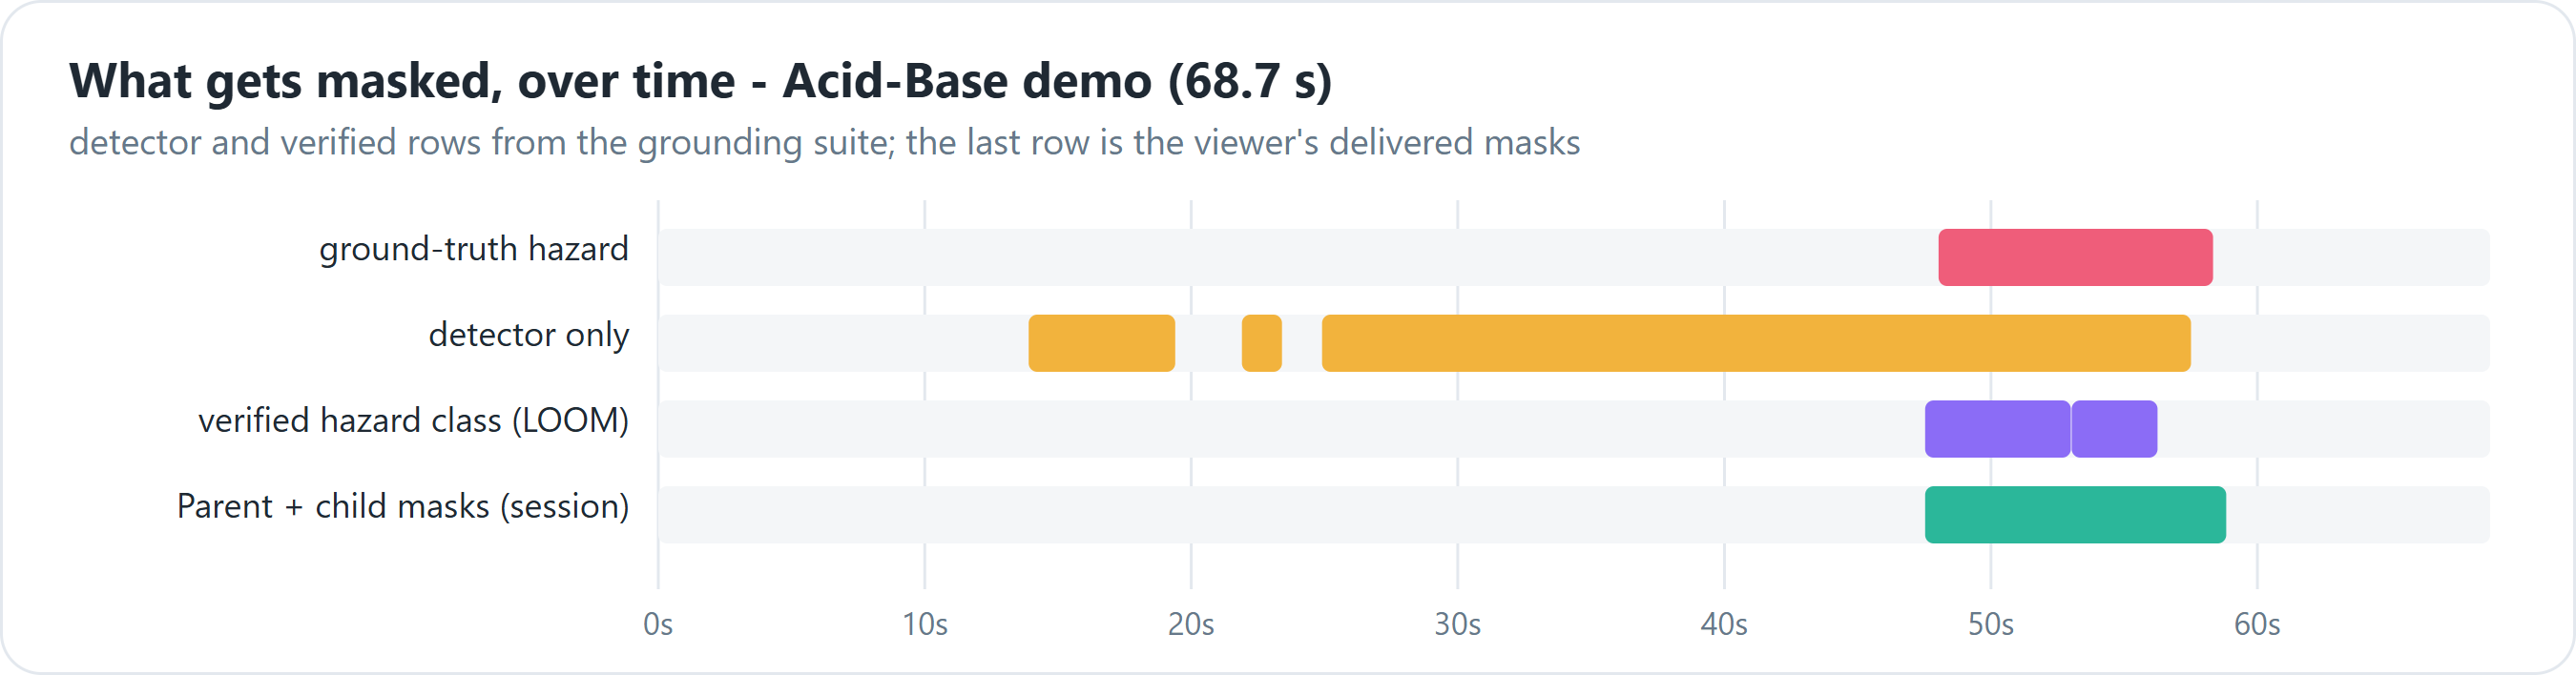
\includegraphics[width=0.49\textwidth]{fig/chart-hazard-timeline-demo.png}\hfill
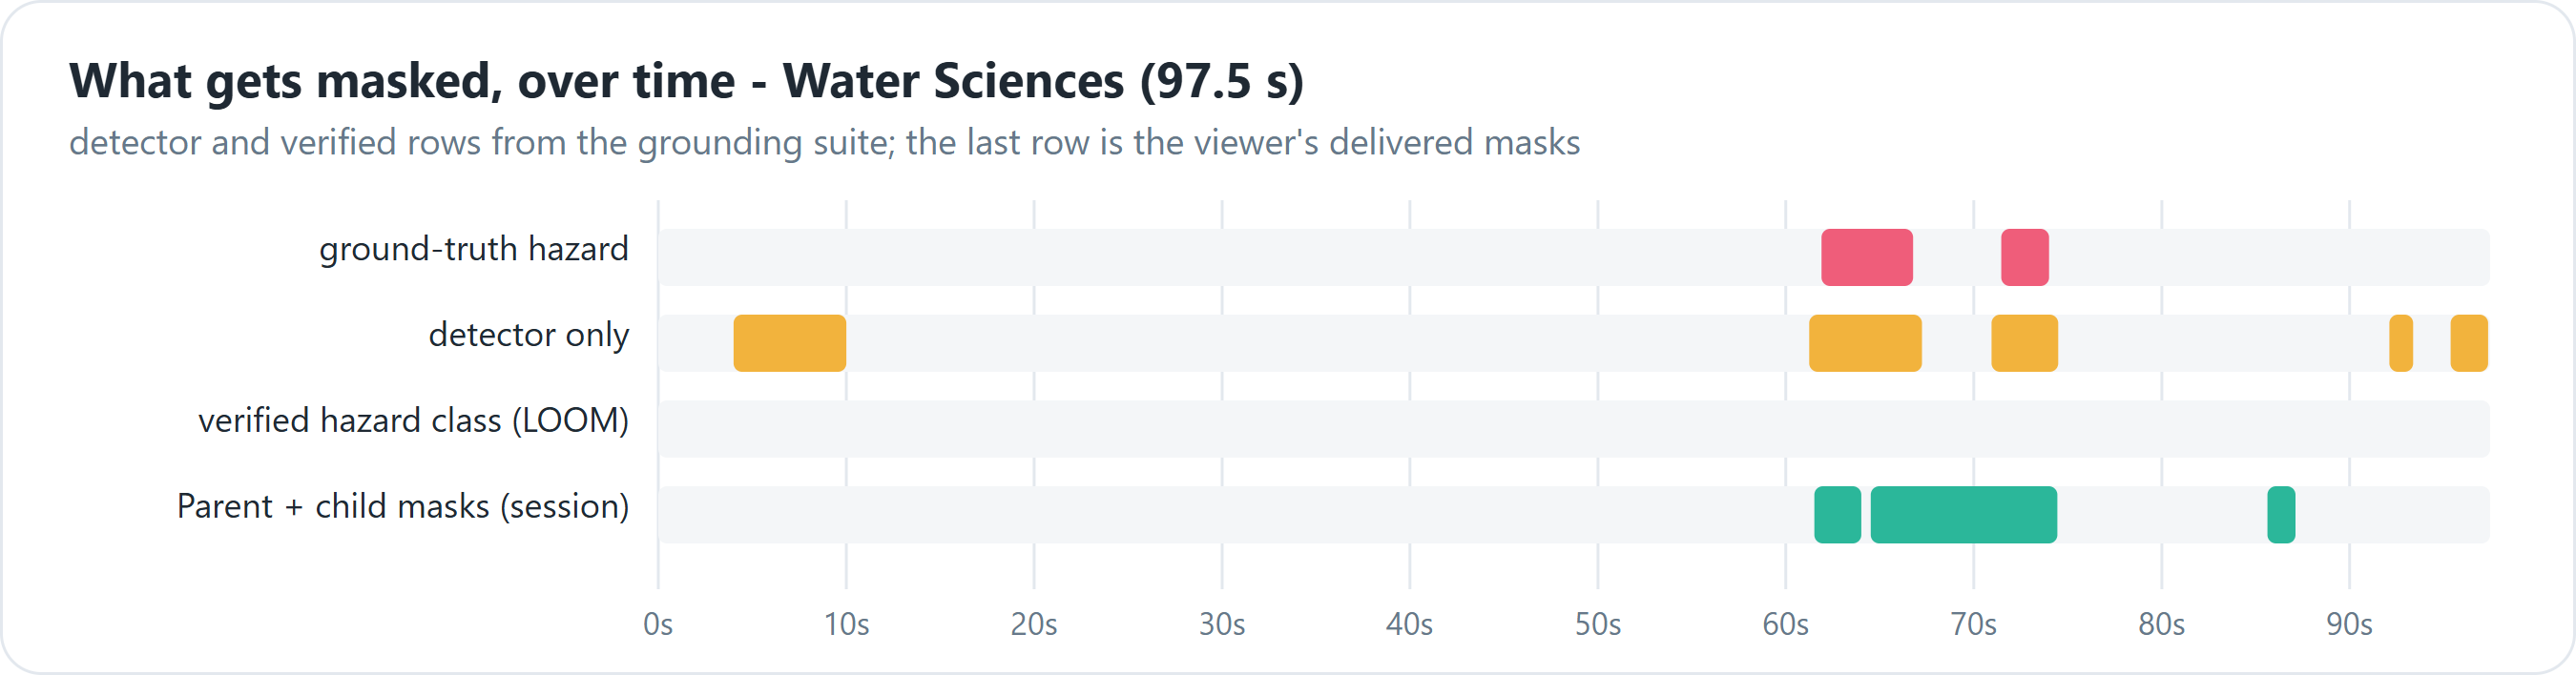
\includegraphics[width=0.49\textwidth]{fig/chart-hazard-timeline-glass.png}
\caption{What is masked over time on the two hazard lessons: ground truth, detector proposals, verified hazard classes
and the Parent\,+\,child viewer's delivered masks (left: demo lesson; right: Water Sciences lesson)}
\label{fig:timelines}
\end{figure}

\subsection{A Second Hazard Lesson}
\label{sec:second}
The Water Sciences lesson shows a broken glass pipette on the floor in two shots (61.9--66.8\,s and 71.5--74.0\,s,
7.4\,s in all). Its window was marked from frame contact sheets at 0.25\,s around each boundary and hard cuts found
from frame differences; a second, independent annotation is pending, so we treat this lesson as a secondary check. The
detector finds the pipette, but as ``cigarette'', ``needle'', ``syringe'' and ``open flame'' (detector-only recall 1.00,
precision 0.39), and both verifiers rightly reject those labels; the vision-language check names it ``pipette''. Class
grounding therefore recalls none of this hazard. The Guardian's review of the tracked ``glass pipette'' object is what
hides it: the Parent\,+\,child cut covers 93\% of the hazard time at 0.5\,s padding, at a precision of 0.50 because it
also masks protective gloves, goggles and a bottle (\fig{fig:timelines}, right). The two safety paths are
complementary; neither is sufficient alone.

\subsection{Redaction and Padding}
Time padding trades precision for recall. On the demo lesson, end-to-end recall rises from 0.505 without padding to
0.796 at 0.5\,s and 0.845 at 1\,s, while precision falls from 1.000 to 0.943 and 0.897. Masks built from the
hand-authored demo graph, which isolates the padding logic from perception, reach recall 1.000 at every setting with
precision 1.000, 0.912 and 0.837. The usual alternative, blocking the whole lesson when it contains a hazard, has recall
1.0 but hides 58.4\,s of safe footage (precision 0.15); the object-mask cut hides 0.5\,s. The comparison is not like for
like, since the object-mask cut misses 20\% of the hazard; on that lesson the remaining misses are small shards that
fly outside the object's mask.

\subsection{Critic Fault Injection}
To test the Critic we plant one fault at a time into the approved cut of each of 3 lessons $\times$ 3 viewers, across
seven families (\tab{tab:faults}, \fig{fig:faults}), and require the expected issue. The Critic detected 76 of 76
planted faults and approved 9 of 9 clean controls. The loop repaired 49; the other 27 ended in the fallback cut, so no
faulty cut was delivered. A further 41 fault--viewer pairs were not applicable (an expert has no unmastered prerequisite
to drop). This is a fire drill, not a measure of real fault rates. It exposed two limits: the loop cannot re-select a
quiz, so factuality and completeness faults always fall back, and the overlap repair can cut a thread mid-sentence,
whose own repair recreates the overlap until the budget runs out.

\begin{table}[t]
\caption{Critic fault injection by family (3 lessons $\times$ 3 viewers)}
\label{tab:faults}
\centering
\begin{tabular}{|l|L{6.2cm}|c|c|c|}
\hline
Family & Planted fault & Injected & Detected & Repaired in loop\\
\hline
F1 structure & overlap, out of order, empty cut & 27 & 27 & 18\\
F2 sentence & condensed end mid-sentence (3 positions) & 18 & 18 & 18\\
F3 factuality & quiz item outside the verified bank & 9 & 9 & 0\\
F4 prerequisite & unmastered prerequisite dropped & 2 & 2 & 2\\
F5 safety & no masks; masks end 1\,s early; mask on the wrong object & 8 & 8 & 8\\
F6 explainer & verified explainer missing & 3 & 3 & 3\\
F8 completeness & empty quiz with a non-empty bank & 9 & 9 & 0\\
\hline
\multicolumn{2}{|l|}{Total (unrepaired faults end in the fallback cut)} & 76 & 76 & 49\\
\hline
\end{tabular}
\end{table}

\begin{figure}[t]
\centering
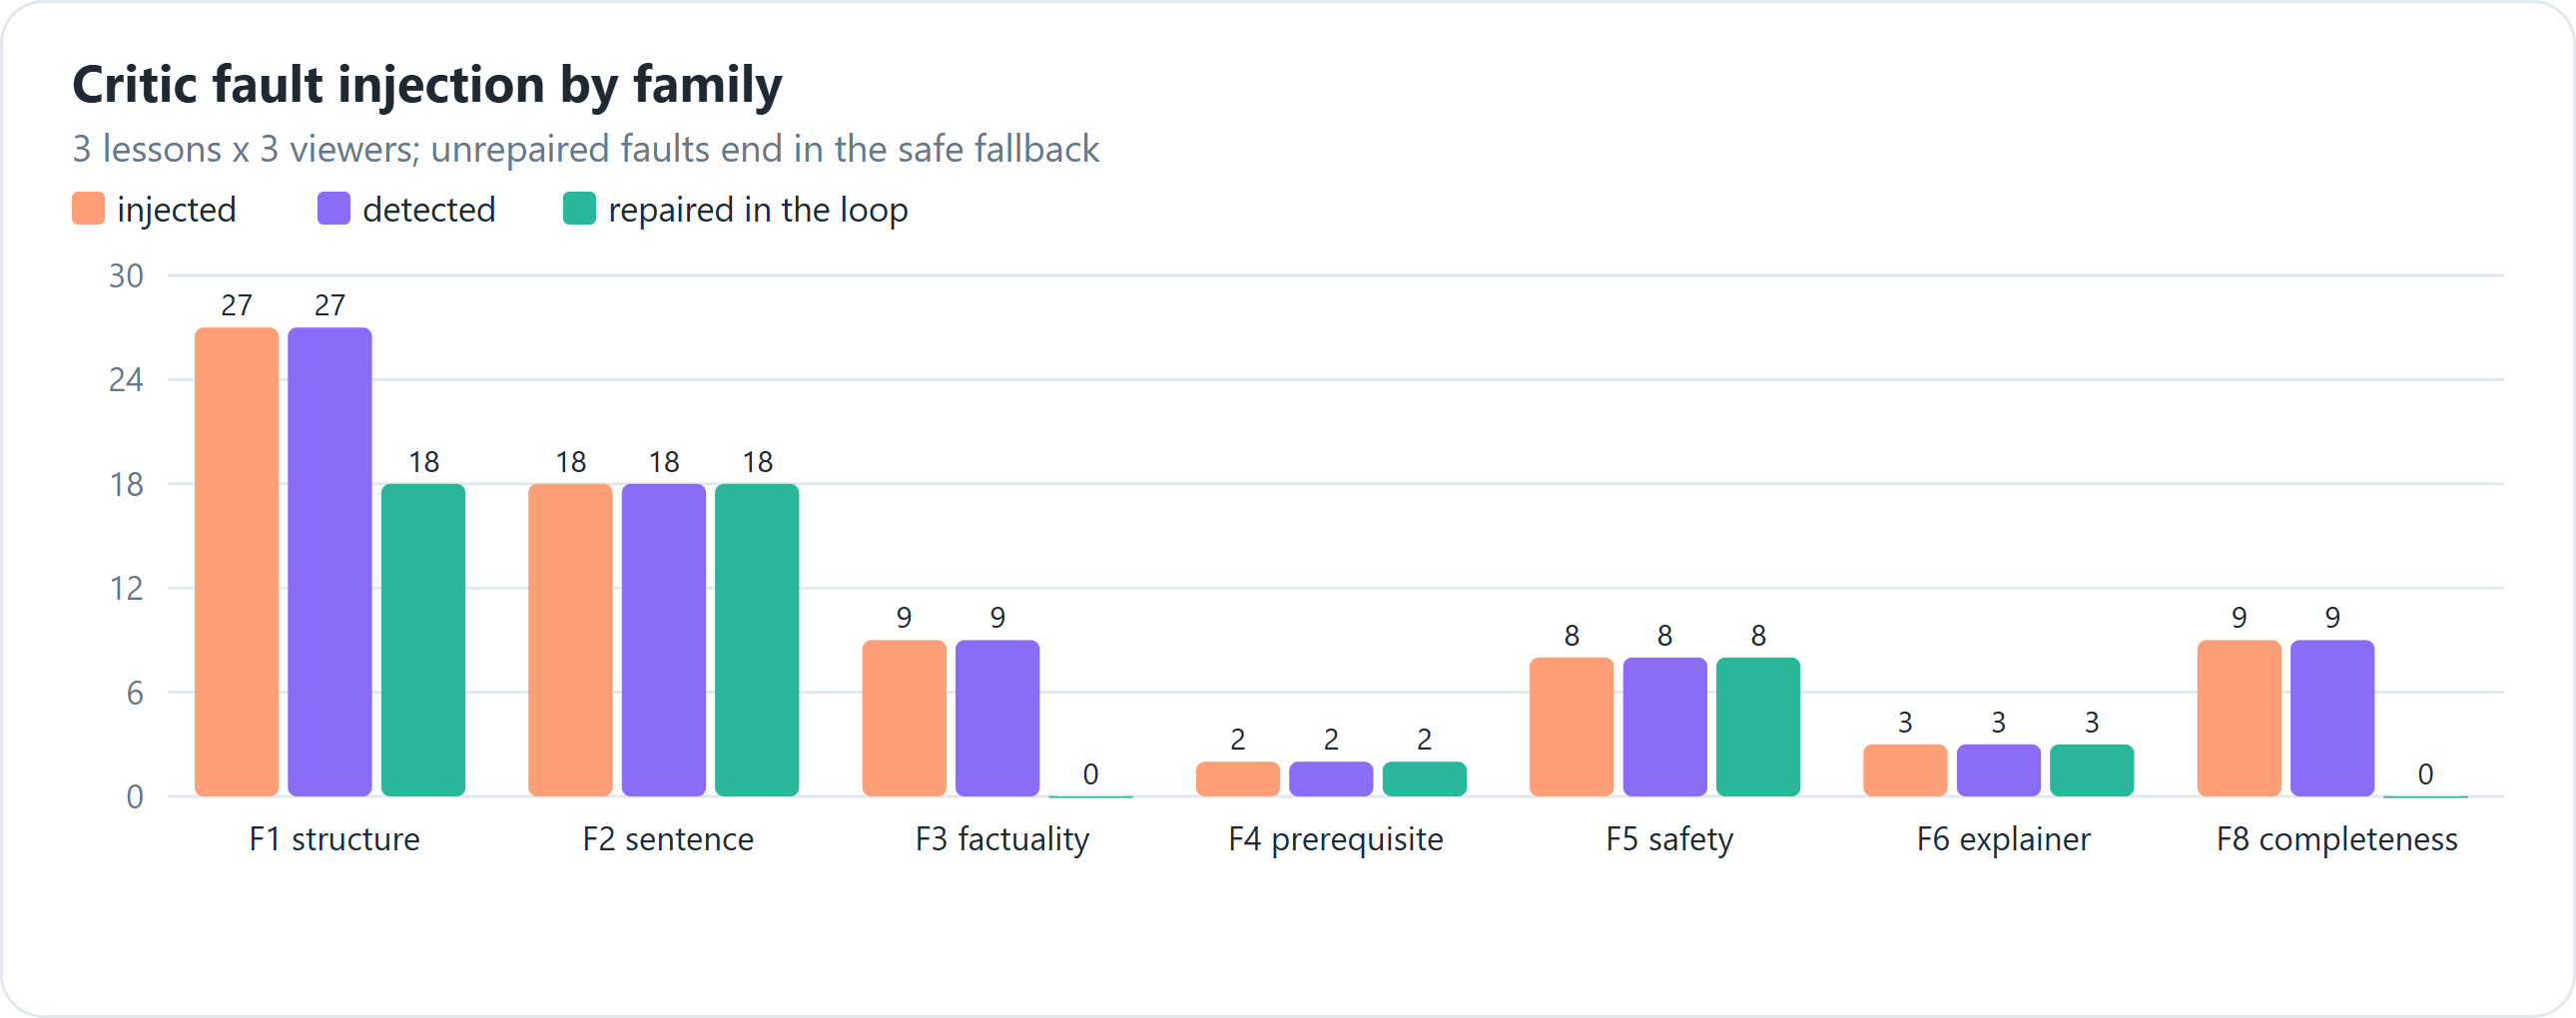
\includegraphics[width=0.49\textwidth]{fig/chart-critic-faults.png}\hfill
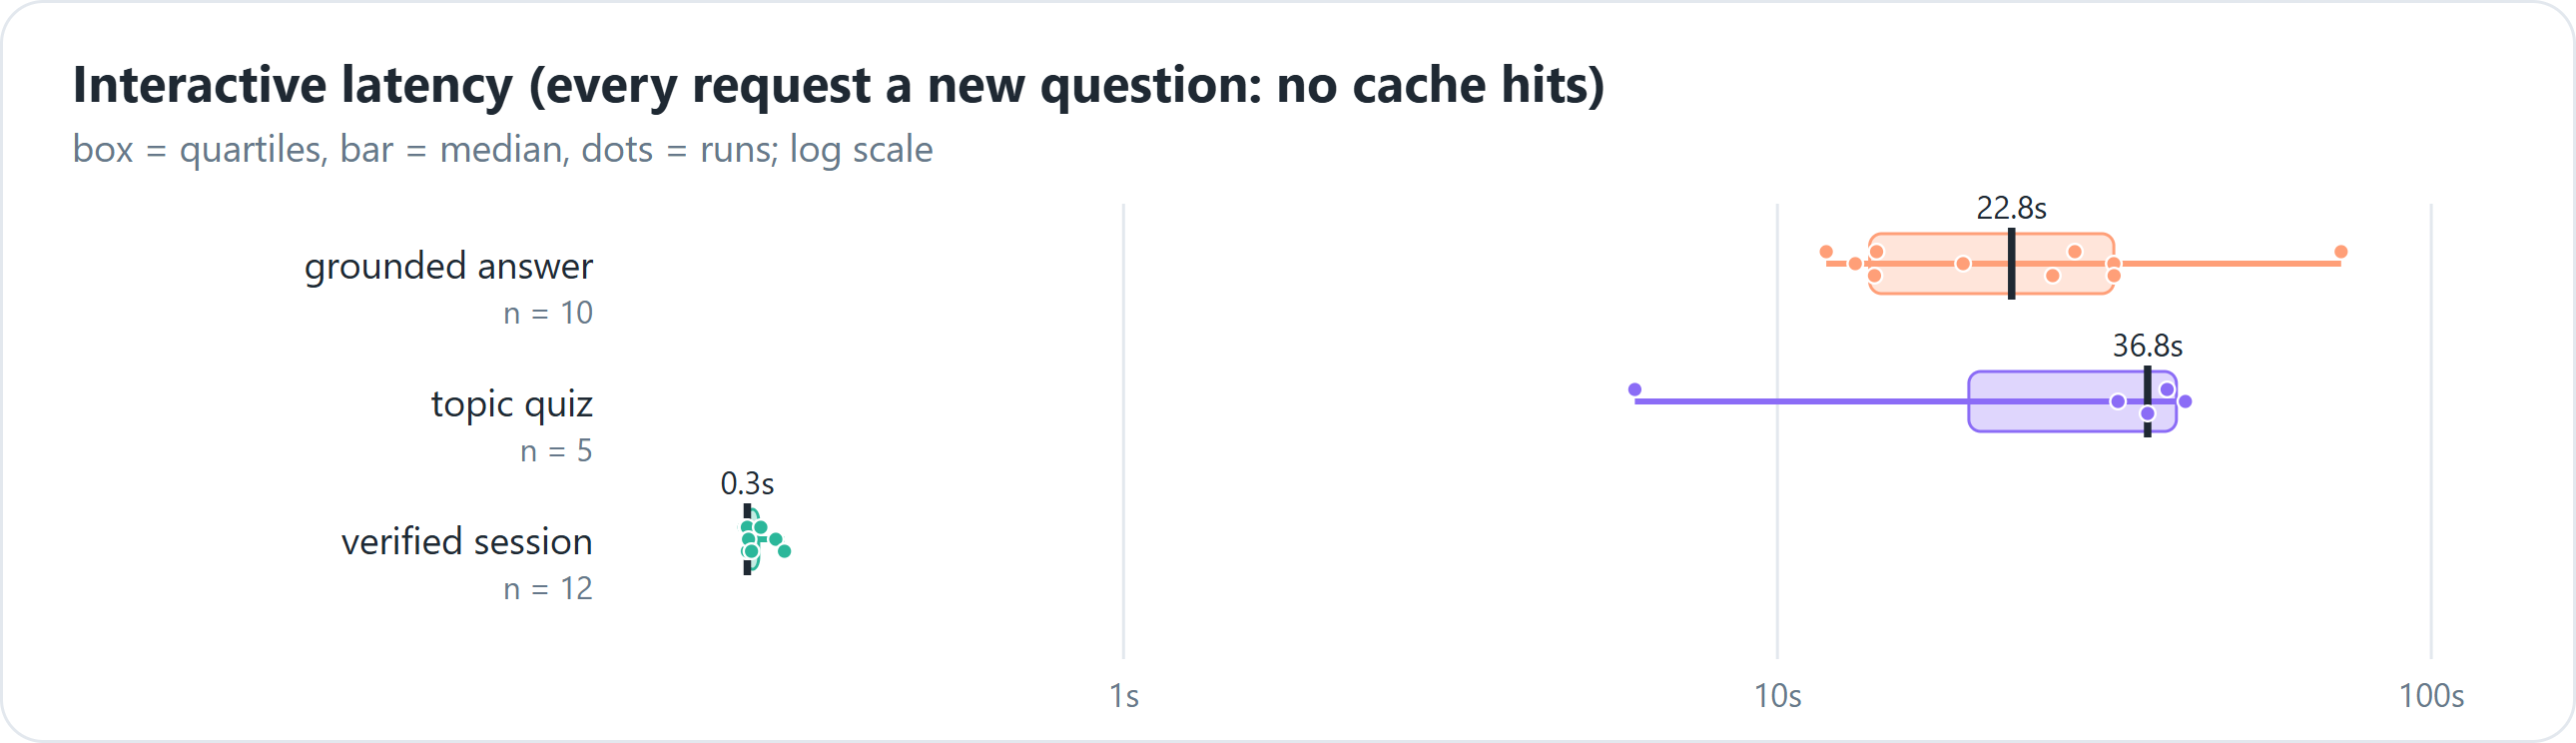
\includegraphics[width=0.49\textwidth]{fig/chart-latency.png}
\caption{Left: Critic fault injection by family (planted, detected, repaired in the loop). Right: interactive latency
over repeated runs (box: quartiles; bar: median; dots: runs; logarithmic scale)}
\label{fig:faults}
\end{figure}

\subsection{Explainers}
In a small trial during development, free-form Manim code from the 9B model rendered in 0 of 8 attempts while
plan-compiled scenes rendered in 3 of 3; this is anecdotal. In the event log, 12 explainer requests delivered 9: the
first draft was fully supported in 5 and accepted after cuts in 9, with 72\% of its 82 lines supported. The
construction mode was added after a geometry request produced a scene of unlabelled spheres; the solver now verifies
such plans before they are drawn (\fig{fig:construct}).

\subsection{Latency, Memory and Cost}
Every request asks a new question, so that no answer comes from the cache (\fig{fig:faults}, right). A grounded answer
through the A2A retriever has a median of 22.8\,s (interquartile range 13.8--32.7\,s, maximum 72.7\,s, $n=10$) and a
topic quiz 36.8\,s (19.6--40.7\,s, $n=5$). Building a verified session takes 0.27\,s ($n=12$, all approved, 10 in one
pass and 2 in two) because the mesh is deterministic; a repeated question is served from the cache in 0.08\,s. The
one-time cost is perception: a median of 11.9\,min per minute of video over 35 stored lessons, dominated by reading each
board element with the vision-language model (43\% of perception time in the breadth run), the quiz stage (12\%) and
fusion (8\%). This is slow for a long lecture but is paid once per lesson.

\subsection{Breadth over 22 Lessons}
To check that the pipeline is not tuned to the corpus, we submitted 30 short public lessons in 14 styles; 22 finished,
covering 12 styles (\tab{tab:breadth}). They yielded 850 tracked elements (38.6 per lesson), 203 named parts, 88
concepts and 106 verified quiz questions, and the answer agent grounded its reply in the video for 21 of 21 lessons
asked. Eight lessons did not finish: four downloads were refused (HTTP 403), one whiteboard animation timed out after
40\,min, and three hit validation bugs that are now fixed. The run also exposed a caption read as one element per
letter; with the overlay fix, a replay of the board scanner on that lesson drops from 43 to 13 elements. These lessons
have no ground truth, so the run shows coverage, not accuracy.

\begin{table}[t]
\caption{Breadth run: mean per lesson by style}
\label{tab:breadth}
\centering
\begin{tabular}{|l|c|c|c|c|c|c|}
\hline
Style & Lessons & Length (s) & Elements & Parts & Concepts & Quiz\\
\hline
Math animation & 4 & 44 & 35.0 & 4.8 & 5.2 & 4.5\\
Chalkboard & 3 & 21 & 20.0 & 2.3 & 2.0 & 2.3\\
2-D explainer & 3 & 50 & 63.0 & 11.7 & 5.7 & 9.7\\
Algorithm visualisation & 2 & 41 & 71.0 & 49.5 & 4.0 & 9.5\\
Data structure & 2 & 26 & 32.0 & 4.5 & 4.0 & 0.0\\
3-D anatomy & 2 & 19 & 0.0 & 0.0 & 3.0 & 0.0\\
Six single-lesson styles$^{a}$ & 6 & 56 & 42.5 & 5.7 & 3.7 & 5.5\\
\hline
\multicolumn{7}{|l|}{\footnotesize $^{a}$Digital whiteboard, glass lightboard, handwriting, chemistry lab, physics demo and coding screencast.}\\
\hline
\end{tabular}
\end{table}

\subsection{Personalisation Outcome}
\fig{fig:cuts} shows the three verified cuts of the demo lesson. Alex (an expert) receives 67\% of the source with no
explainer and no mask; Priya (a beginner) receives 100\% with two explainers; the Parent\,+\,child viewer receives 98\%
with one mask over the broken-glass segment. Each cut was approved on the first pass, with three questions each.

\begin{figure}[t]
\centering
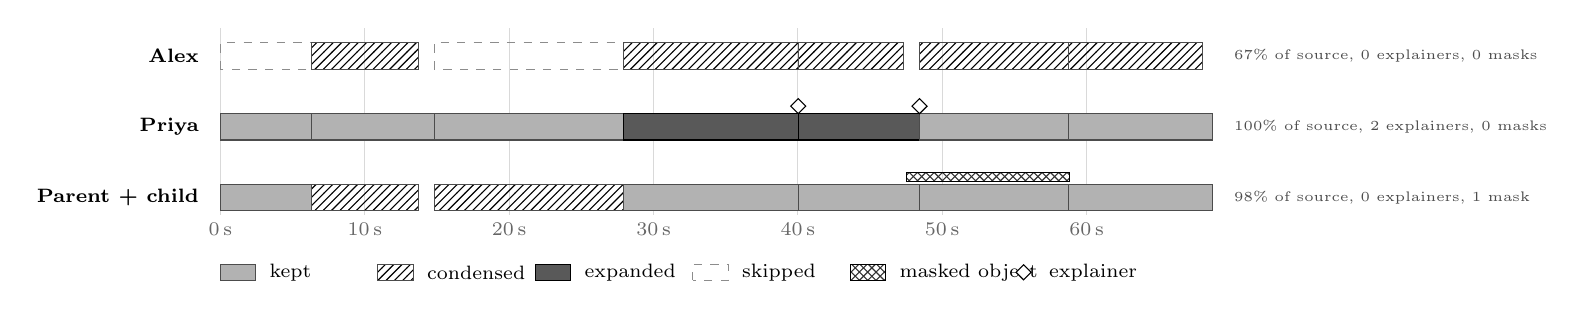
\begin{tikzpicture}[font=\scriptsize]
\tikzset{keep/.style={fill=black!30, draw=black!70}, condense/.style={pattern=north east lines, draw=black!70}, expand/.style={fill=black!65, draw=black}, skipped/.style={draw=black!45, dashed}, mask/.style={pattern=crosshatch, pattern color=black!80, draw=black}}
\draw[black!15] (0.000,0.35) -- (0.000,-2.02); \node[black!60] at (0.000,-2.2) {0\,s};
\draw[black!15] (1.833,0.35) -- (1.833,-2.02); \node[black!60] at (1.833,-2.2) {10\,s};
\draw[black!15] (3.666,0.35) -- (3.666,-2.02); \node[black!60] at (3.666,-2.2) {20\,s};
\draw[black!15] (5.500,0.35) -- (5.500,-2.02); \node[black!60] at (5.500,-2.2) {30\,s};
\draw[black!15] (7.333,0.35) -- (7.333,-2.02); \node[black!60] at (7.333,-2.2) {40\,s};
\draw[black!15] (9.166,0.35) -- (9.166,-2.02); \node[black!60] at (9.166,-2.2) {50\,s};
\draw[black!15] (10.999,0.35) -- (10.999,-2.02); \node[black!60] at (10.999,-2.2) {60\,s};
\node[anchor=east, align=right, font=\scriptsize\bfseries] at (-0.15,0.00) {Alex};
\node[anchor=west, font=\tiny, black!70] at (12.75,0.00) {67\% of source, 0 explainers, 0 masks};
\draw[skipped] (0.000,-0.17) rectangle (1.155,0.17);
\draw[skipped] (2.713,-0.17) rectangle (5.120,0.17);
\draw[condense] (1.155,-0.17) rectangle (2.510,0.17);
\draw[condense] (5.120,-0.17) rectangle (7.338,0.17);
\draw[condense] (7.338,-0.17) rectangle (8.675,0.17);
\draw[condense] (8.878,-0.17) rectangle (10.766,0.17);
\draw[condense] (10.766,-0.17) rectangle (12.469,0.17);
\node[anchor=east, align=right, font=\scriptsize\bfseries] at (-0.15,-0.90) {Priya};
\node[anchor=west, font=\tiny, black!70] at (12.75,-0.90) {100\% of source, 2 explainers, 0 masks};
\draw[keep] (0.000,-1.07) rectangle (1.155,-0.73);
\draw[keep] (1.155,-1.07) rectangle (2.713,-0.73);
\draw[keep] (2.713,-1.07) rectangle (5.120,-0.73);
\draw[expand] (5.120,-1.07) rectangle (7.338,-0.73);
\draw[expand] (7.338,-1.07) rectangle (8.878,-0.73);
\draw[keep] (8.878,-1.07) rectangle (10.766,-0.73);
\draw[keep] (10.766,-1.07) rectangle (12.600,-0.73);
\node[draw, fill=white, diamond, inner sep=1.4pt] at (7.338,-0.64) {};
\node[draw, fill=white, diamond, inner sep=1.4pt] at (8.878,-0.64) {};
\node[anchor=east, align=right, font=\scriptsize\bfseries] at (-0.15,-1.80) {Parent + child};
\node[anchor=west, font=\tiny, black!70] at (12.75,-1.80) {98\% of source, 0 explainers, 1 mask};
\draw[keep] (0.000,-1.97) rectangle (1.155,-1.63);
\draw[condense] (1.155,-1.97) rectangle (2.510,-1.63);
\draw[condense] (2.713,-1.97) rectangle (5.120,-1.63);
\draw[keep] (5.120,-1.97) rectangle (7.338,-1.63);
\draw[keep] (7.338,-1.97) rectangle (8.878,-1.63);
\draw[keep] (8.878,-1.97) rectangle (10.766,-1.63);
\draw[keep] (10.766,-1.97) rectangle (12.600,-1.63);
\draw[mask] (8.713,-1.60) rectangle (10.785,-1.48);
\draw[keep] (0.00,-2.85) rectangle (0.45,-2.65); \node[anchor=west] at (0.50,-2.75) {kept};
\draw[condense] (2.00,-2.85) rectangle (2.45,-2.65); \node[anchor=west] at (2.50,-2.75) {condensed};
\draw[expand] (4.00,-2.85) rectangle (4.45,-2.65); \node[anchor=west] at (4.50,-2.75) {expanded};
\draw[skipped] (6.00,-2.85) rectangle (6.45,-2.65); \node[anchor=west] at (6.50,-2.75) {skipped};
\draw[mask] (8.00,-2.85) rectangle (8.45,-2.65); \node[anchor=west] at (8.50,-2.75) {masked object};
\node[draw, fill=white, diamond, inner sep=1.4pt] at (10.20,-2.75) {}; \node[anchor=west] at (10.40,-2.75) {explainer};
\end{tikzpicture}
\caption{Three verified cuts of the demo lesson over the source timeline, drawn from the stored cuts}
\label{fig:cuts}
\end{figure}

\subsection{Design Alternatives}
\tab{tab:alts} collects the alternatives we measured, with numbers from the sections above and from the model spike.

\begin{table}[t]
\caption{Design choices and measured alternatives}
\label{tab:alts}
\centering
\begin{tabular}{|L{2.4cm}|L{4.6cm}|L{6.3cm}|}
\hline
Decision & Alternative $\rightarrow$ chosen & Measured difference\\
\hline
Hazard rule & AND, VLM only or SigLIP\,2 only $\rightarrow$ OR & F1 0.863 vs 0.254, 0.541 and 0.736\\
Safety paths & class grounding only $\rightarrow$ + Guardian & second lesson: recall 0 $\rightarrow$ 0.93\\
Mask scope & whole lesson $\rightarrow$ objects & 58.4\,s vs 0.5\,s of safe footage hidden\\
Guardian build & Q6\_K $\rightarrow$ q4\_K\_M & Q6\_K spills 2\,GB and is $\sim$4$\times$ slower; same accuracy\\
Brain context & 8192 $\rightarrow$ 6144 tokens & spills 0.79\,GB vs fits in 5.58\,GB\\
Brain mode & thinking $\rightarrow$ off & p50 52.6\,s, valid 0.90 vs 3.5\,s, valid 1.00\\
SAM\,2 run & whole video $\rightarrow$ 20\,s windows & peak memory 8.88\,GB $\rightarrow$ 2.91\,GB\\
Explainer & free-form Manim $\rightarrow$ scene plan & 0 of 8 vs 3 of 3 renders (anecdotal)\\
\hline
\end{tabular}
\end{table}

\section{Discussion}
\emph{RQ1.} All 12 measured sessions were approved within the budget (10 in one pass), and every planted fault was
caught or ended in the fallback, so bounded verified cuts are feasible locally. \emph{RQ2.} Staged verification removes
almost all false blocking (30.1\,s to 0.5\,s) but does not reach the 0.90 recall target; on the second lesson the
per-object safety review, not class grounding, is what finds the hazard. \emph{RQ3.} Plan-compiled scenes rendered
where free-form code did not, and constructions resolve fully, but the comparison is small. \emph{RQ4.} The fact-check
removed lines in most first drafts; whether every removed line was truly unsupported has not been validated against
human judgement. \emph{RQ5.} Every run leaves an event log that the interface replays, and every cited answer links to
its evidence.

The main limitations follow. Hazard recall is below target and the vision-language check is not stable between runs.
The Guardian over-flags protective gear such as gloves and goggles, which hides useful safety information. Hazard ground
truth comes from one synthetic lesson and one secondary lesson, and mask quality has not been measured against
hand-drawn masks. The judge's agreement with human annotators is not yet measured. The loop cannot re-select a quiz.
All results come from one GPU and small test sets, nondeterminism is reduced but not eliminated, and no user study has
asked viewers whether the cuts help them learn.

\emph{Ethics.} All inference is local, with no cloud calls, keys or cloud speech services; lesson footage, transcripts
and viewer mastery stay on the machine. The one network exception is a user-initiated YouTube download (and optional
Wikimedia pictures in explainers), which the offline setting disables. The study involved no human subjects and no
personal data; the viewers are synthetic profiles, and no frames from third-party lessons are reproduced in this paper.
The safety taxonomy and thresholds encode choices about what is unsafe for a child, and protective gear was masked as a
side effect. Detectors and language models may perform unevenly across accents, scripts and drawing styles, which our
small corpus cannot measure. A missed hazard is the most serious error, because a parent may trust the cut; LOOM fails
closed, but delivered recall is below target, so its output is not a guarantee that a lesson is safe for a child.
Over-masking harms learning, so the balance between the two errors should be a setting the parent can see and change.

\section{Conclusions}
LOOM shows that one video can become many verified cuts on a single laptop GPU, with object-level masks, explainers
whose every line is checked, and a Critic that never delivers a cut it could not verify. The Critic caught every planted
fault, staged verification removed almost all false blocking, and two complementary safety paths together found a hazard
that neither found alone; hazard recall still misses its target and perception is slow. Future work will raise recall,
measure mask quality against hand-drawn masks, validate the fact-checker against human judgement, cap the elements read
per lesson, re-run the three lessons that failed on since-fixed bugs, and run a user study with learners and parents.

\section*{Acknowledgment}
The demo lesson uses royalty-free footage from Pexels, and the Water Sciences Laboratory Tutorial is a Creative Commons
YouTube lesson; we thank their creators and the maintainers of the open models used. The authors used an AI coding
assistant during software development, evaluation scripting and language editing; all reported numbers were produced
by the project's evaluation code and checked by the authors, who take full responsibility for the content.

\section*{References}
{\fontsize{8.5}{10}\selectfont
\begin{enumerate}[label={[\arabic*]},leftmargin=*,itemsep=0pt,topsep=2pt]
\item T. Sanal Kumar and R. Thandeeswaran, ``An improved adaptive personalization model for instructional video-based
e-learning environments,'' \emph{J. Comput. Educ.}, 2024, doi: 10.1007/s40692-023-00310-x.
\item G. Hardaker and L. Glenn, ``Artificial intelligence for personalized learning: a systematic literature review,''
\emph{Int. J. Inf. Learn. Technol.}, 2025, doi: 10.1108/IJILT-07-2024-0160.
\item A. Cattaneo, H. van der Meij, C. Aprea, F. Sauli, and C. Zahn, ``A model for designing hypervideo-based
instructional scenarios,'' \emph{Interact. Learn. Environ.}, vol. 27, no. 4, pp. 508--529, 2019, doi:
10.1080/10494820.2018.1486860.
\item M. Chuttur and A. Nazurally, ``A multi-modal approach to detect inappropriate cartoon video contents using deep
learning networks,'' \emph{Multimed. Tools Appl.}, 2022, doi: 10.1007/s11042-022-12709-2.
\item K. Yousaf and T. Nawaz, ``A deep learning-based approach for inappropriate content detection and classification
of YouTube videos,'' \emph{IEEE Access}, vol. 10, 2022, doi: 10.1109/ACCESS.2022.3147519.
\item ``Agent2Agent (A2A) protocol specification,'' \url{https://a2a-protocol.org} (accessed Nov. 2026).
\item T. Wang \emph{et al.}, ``LLM-powered multi-agent framework for goal-oriented learning in intelligent tutoring
system,'' in \emph{Proc. ACM Web Conf. 2025, Industry Track}, arXiv:2501.15749.
\item X. Zhang \emph{et al.}, ``EduPlanner: LLM-based multiagent systems for customized and intelligent instructional
design,'' \emph{IEEE Trans. Learn. Technol.}, 2025, doi: 10.1109/TLT.2025.3561332.
\item M. Chakraborty \emph{et al.}, ``PAL: Personal adaptive learner,'' in \emph{Proc. AAAI Conf. Artif. Intell.}, vol.
40, 2026, doi: 10.1609/aaai.v40i48.42337.
\item A. Madaan \emph{et al.}, ``Self-Refine: Iterative refinement with self-feedback,'' in \emph{Proc. NeurIPS}, vol.
36, 2023.
\item L. Zheng \emph{et al.}, ``Judging LLM-as-a-judge with MT-Bench and Chatbot Arena,'' in \emph{Proc. NeurIPS
Datasets and Benchmarks Track}, 2023.
\item B. Castellano, ``PySceneDetect,'' \url{https://www.scenedetect.com}.
\item A. Radford, J. W. Kim, T. Xu, G. Brockman, C. McLeavey, and I. Sutskever, ``Robust speech recognition via
large-scale weak supervision,'' in \emph{Proc. ICML}, PMLR vol. 202, 2023, pp. 28492--28518.
\item RapidAI, ``RapidOCR,'' \url{https://github.com/RapidAI/RapidOCR}.
\item S. Liu \emph{et al.}, ``Grounding DINO: Marrying DINO with grounded pre-training for open-set object detection,''
in \emph{Proc. ECCV}, 2024, doi: 10.1007/978-3-031-72970-6\_3.
\item M. Li \emph{et al.}, ``Qwen3 Embedding: Advancing text embedding and reranking through foundation models,''
arXiv:2506.05176, 2025.
\item N. Ravi \emph{et al.}, ``SAM 2: Segment anything in images and videos,'' in \emph{Proc. ICLR}, 2025,
arXiv:2408.00714.
\item M. Tschannen \emph{et al.}, ``SigLIP 2: Multilingual vision-language encoders with improved semantic
understanding, localization, and dense features,'' arXiv:2502.14786, 2025.
\item I. Padhi \emph{et al.}, ``Granite Guardian,'' arXiv:2412.07724, 2024.
\item J. Yang, H. Zhang, F. Li, X. Zou, C. Li, and J. Gao, ``Set-of-Mark prompting unleashes extraordinary visual
grounding in GPT-4V,'' arXiv:2310.11441, 2023.
\item hexgrad, ``Kokoro-82M,'' \url{https://huggingface.co/hexgrad/Kokoro-82M}.
\item The Manim Community Developers, ``Manim -- mathematical animation framework,'' \url{https://www.manim.community}.
\item Google DeepMind, ``Gemma open models,'' \url{https://ai.google.dev/gemma}.
\item A. Yang \emph{et al.}, ``Qwen3 technical report,'' arXiv:2505.09388, 2025.
\item Zhipu AI, ``GLM-OCR,'' \url{https://ollama.com/library/glm-ocr}.
\end{enumerate}}

\end{document}
